\documentclass[a4paper,10pt]{article}
\usepackage[utf8x]{inputenc}
\usepackage{amsmath,amsthm,amssymb}
\usepackage[pdftex,backref=page,hyperfigures,breaklinks,colorlinks]{hyperref}
\usepackage{graphicx}

\newcommand{\mdp}{\textsc{Mdp}}
\newcommand{\mdps}{\textsc{Mdp}s}
\renewcommand{\abstractname}{Summary}

% Title Page
\title{Integrating MDPs into Gujarat Simulation}
\author{Miquel Ramírez}

\begin{document}
\maketitle

\begin{abstract}
This document describes how Monte--Carlo Tree Search techniques have been introduced into
the Gujarat Simulation in order to control hunter gatherer agents. New concepts introduced
into the framework will be introduced, along with the new classes and interfaces which encode
these concepts and the changes made in existing code in order to accomodate them into the existing
system. Implementation notes will be offered which will cover those aspects critical
for performance and soundness. The last section in this document contains a \textsc{To--Do} list, which
should be taken as the roadmap for future steps.
\end{abstract}

\tableofcontents

\section{Monte--Carlo Tree Search and MDPs}

Given the complexity of the Gujarat agent--based simulation, we have discarded out of hand model--based approaches
to solve \mdps, as the ones discussed in the classical Optimal Foraging Theory literature. Rather than attempting
at computing a value function $V$, and therefore a policy $\pi_{V}$, out of the \mdp~ model $M$, either with 
\emph{model--based} algorithms such as Value Iteration, we have aimed at obtaining an on--line \emph{action selection} 
mechanism, which \emph{implicitly} defines a policy $\pi$ for \mdp~$M$.

These family of algorithms, collectively known as \emph{simulation--based}, do not require a full model of the \mdp~$M$
but it rather suffices that the algorithm has access to a simulation of $M$ which allows it to \emph{sample} the state
space and the outcomes of actions. In the context of the Gujarat simulation, this amounts to provide an interface so
that relevant parts of the agent--based simulation are made available to a component simulating the \mdp~$M$. So far,
this has proved to be a relatively easy task.

\section{New Concepts, Classes \& Interfaces Introduced}

We have taken Blai Bonet's \texttt{libmdp} library concepts and implementation of algorithms off--the--shelf and 
integrated it into the Gujarat simulation, including suitably defined implementations of the interfaces 
in \texttt{libmdp} for the concepts of \textsc{State} and \textsc{Model} and creating a \emph{proxy} interface
\textsc{AgentController} that allows to abstract away the details of how agents in the simulation choose actions.

When this mechanism relies on action selection algorithms for \mdps, the concrete controller amounts to wrap together
the \mdp~model object, which is sort of an \emph{observer} on \textsc{GujaratAgent} objects, with the selected
simulation--based \mdp~algorithm. In the current implementation we are using the implementation of \textsc{Uct} available
on \texttt{libmdp}.

Finally, a class encapsulating the parameters which can be tweaked from the simulation \textsc{Xml} configuration
document, has been introduced. This allows to put some order into the the sorry mess that the \textsc{GujaratConfig}
class is becoming as we progress.

\begin{figure}[htbp]
\centering
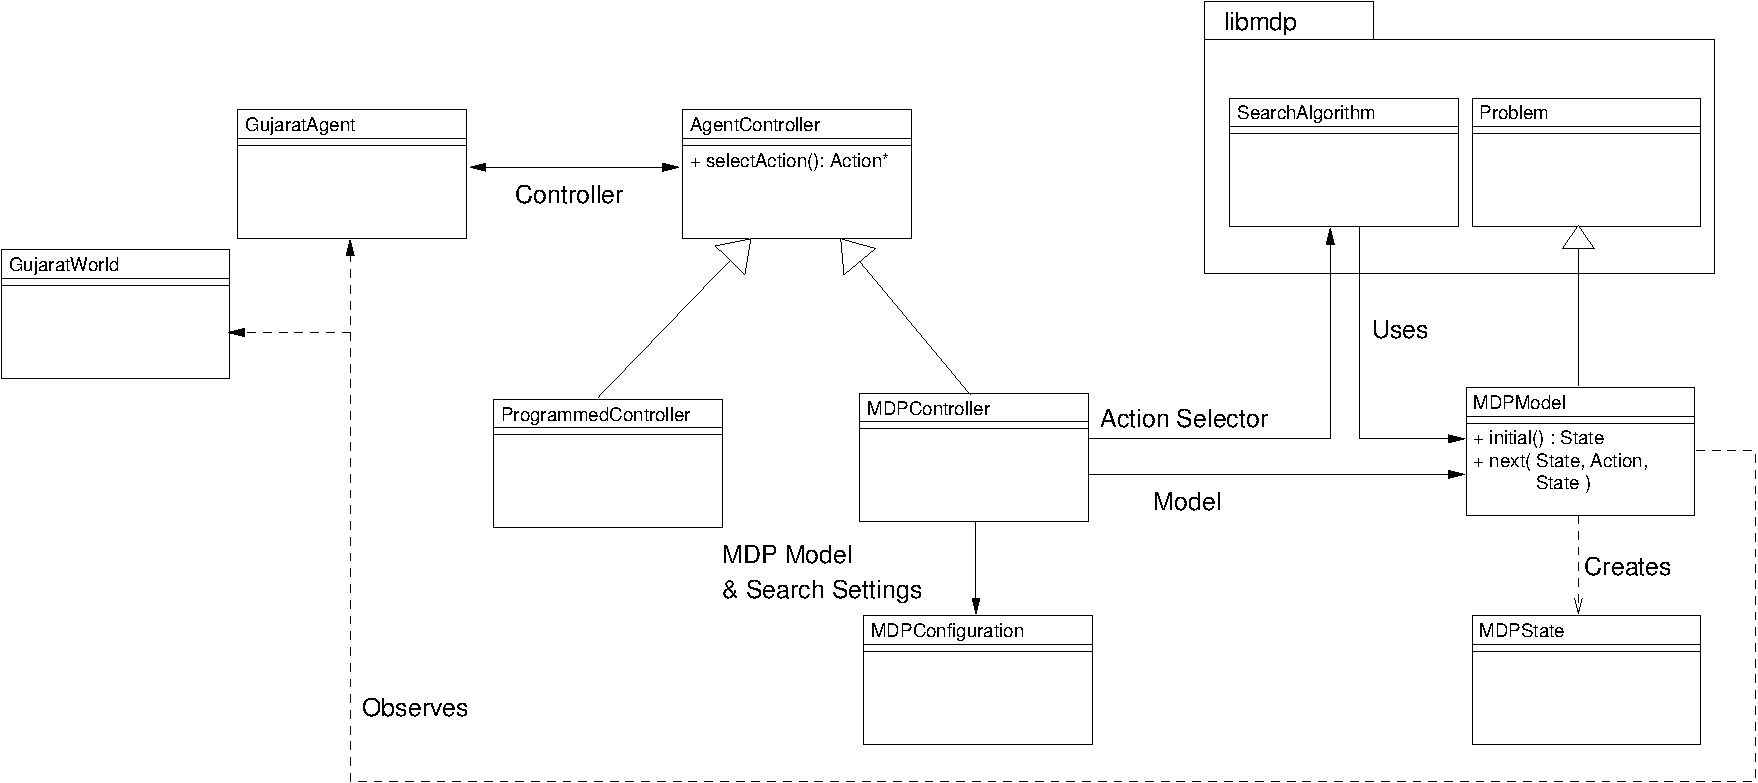
\includegraphics[scale=0.65,keepaspectratio,angle=90]{static-view.pdf}
\label{static-view}
\caption{Overview of the integration between the Gujarat simulation and \texttt{libmdp}.}
\end{figure}

A general overview of the relationships and interaction of the new components between them and with already existing
components such as \textsc{GujaratAgent} or \textsc{GujaratWorld} is depicted in Figure~\ref{static-view}.

\subsection{MDP Configuration}

This class implementation resides on the files:
\begin{itemize}
\item \texttt{HunterGathererMDPConfig.hxx}
\item \texttt{HunterGathererMDPConfig.cxx}
\end{itemize}

For now, we are exposing four parameters:

\begin{itemize}
 \item \emph{Number of \textsc{Forage} actions} -- This allows to further restrict the number of \textsc{Forage} actions
to be considered beyond the restriction inherent in the number of sectors which model the Hunter--Gatherer agent perception
of her environment. Since we are already ranking these \textsc{Forage} actions, I doubt that every action is actually required
to be evaluated. This should allow us to restrict the branching factor of the state space and avoid performing unnecessary
computation. This value \textbf{cannot} be bigger than the number of sectors specified in the Hunter--Gatherer configuration.
\item \emph{Number of \textsc{MoveHome} actions} -- Similarly to the above, the ranking we are doing on 
\textsc{SettlementAreas} opens up the possibility of more aggressive simplification. The value of this parameter is not
constrained by any other parameters in the \textsc{Xml} configuration. If this value is higher than the actual number of
\textsc{SettlementAreas} found to be relevant for an agent during the simulation, no additional ``virtual'' actions are
generated.
\item \emph{Do Nothing Is Allowed} -- While we are pretty confident on the \textsc{Forage} and \textsc{MoveHome} actions,
the issue raised by M. Madella regarding hunter--gatherers -- in the real world -- not foraging or moving around all the
time is valid. However, we have very little meaning attached to this action. We don't really have any \emph{incentives}
in the simulation for the agent to do this, that is, to do nothing at all. Perhaps this could model other activities
such as mending hunting equipment. But it also sort of overlaps with the yet--to--be--introduced \emph{social} activities
we have in our draft design document.
\item \emph{Horizon} -- The number of time steps in the \mdp~$M$. This refers to the notion of the agent deliberating,
by means of projecting itself and the outcome of its future actions forward in time. In principle, the bigger this
horizon $T$ is, the \emph{better} informed will be the decisions the agent makes. However, this comes at a hefty
computational cost. On the other hand, this parameter can also model cognitive limitations inherent to human decision--making.
\end{itemize}


\subsection{MDP State}

This class implementation resides on the files:
\begin{itemize}
\item \texttt{HunterGathererMDPState.hxx}
\item \texttt{HunterGatehrerMDPState.cxx}
\end{itemize}

This is a subclass of \texttt{libmdp} \textsc{State} interface. Initial states $s_0$ are a \emph{view} on the Gujarat simulation
state when an action is requested from an agent at simulation step $t$. Three datums are extracted from the simulation state:
\begin{itemize}
\item The \emph{resources} dynamic raster state at simulation step $t$.
\item The location on the map of the agent.
\item The amount of calories the agent has \emph{on hand} at simulation step $t$.
\end{itemize}
The reason for these datums to be extracted is that these are the elements of the simulation state which are \emph{directly}
modified by the three actions we are considering for Hunter--Gatherer agents, namely, \textsc{Forage}, \textsc{MoveHome}
and \textsc{DoNothing}. States $s$ resulting from applying any action $a$, can be formally defined as follows
\begin{equation*}
\langle R,\ \vec{l}, C, d \rangle
\end{equation*}
where $R$ is the resource raster resulting from applying any actions, $\vec{l}$ is the location of the agent, $C$ is
the number of calories the agent has \emph{on hand} and $d$ is the associated time index. While $\vec{l}$ and $C$ are
very light objects -- primitive types or collections of such -- the resources raster is a potentially huge collection
of values\footnote{Right now we are working with a ``toy'' $400$x$400$ grid, which is already rather big.}. This involved
introducing the class \textsc{IncrementalRaster}, a subclass of \textsc{Raster} which is 
discussed on Section~\ref{lw_states}. Another important issue is that of \emph{hashing} states, important to detect
``duplicate'' states, that it, states resulting from actions $a$ and $b$ at time step $d$ which result in the same
value for $R$, $\vec{l}$ and $C$. Hashing is discussed in Section~\ref{states_hashing}.

States are \emph{terminal states} whenever the value of the time index equals that of the horizon, $d=T$. For now we are
leaving out the possibility of the agent dying or emigrating during the next $T$ simulation time steps\footnote{Actually
this is an application of the ``optimism in the face of uncertainty'' heuristic. Note that heuristics can be either
used \emph{implicitly} during modeling, that is, the modeller ``hardcodes'' the heuristic, or made \emph{explicit} by 
analyzing the structure of some given model so it can be exploited computationally.}.

I have decided to store the actions applicable to an state $s$ in the \textsc{State} object itself as it is the most
compact way to deal with state spaces where states may have very different numbers and kinds of actions being applicable.
This adds some complexity to the implementation of actions (see Section~\ref{changes_actions}) and that of the \textsc{State}
class itself, since copy constructors need to be implemented carefully and make sure that copies of \textsc{State} objects
keep valid pointers to action objects at all times.

\subsection{MDP Model}
\label{mdp_model}
The implementation of the class encapsulating the notion of \mdp~model or \emph{problem} can be found on this
two files:
\begin{itemize}
\item \texttt{HunterGathererMDPModel.hxx}
\item \texttt{HunterGathererMDPModel.cxx}
\end{itemize}

This class has two roles. On the one hand, it fulfills the \emph{Observer} pattern, by associating itself with one
of the Hunter--Gatherer agents currently active in the simulation. On the other hand, it fulfills the \emph{Facade}
pattern, providing the action selection algorithm with access to states and the transition function. We will devote
some space to discuss successor state generation.

Whenever an action is executed on a \textsc{State} object, representing an \mdp~state $s$, the \texttt{next()} method
is invoked in order to obtain a second \textsc{State} object, which corresponds to one state $s' \in F(s,a)$, where
$F(\cdot)$ is a non--deterministic transition function. In our case, $F(\cdot)$ is implemented on top of the same
elements as actions are \emph{actually} executed on simulation states. This function is not deterministic since the
\textsc{Forage} action effects include \emph{chance} outcomes, such as the actual amount of biomass retrieved from
cells in a given \textsc{Sector}.

Generating $s'$ consists of three steps, which are implemented in different places:
\begin{enumerate}
\item The \textsc{State} class, which has the responsability of properly initializing $s'$ attributes in terms of
the attributes of $s$.
\item Concrete \textsc{Action} class, which modifies $s'$ attributes as necessary to account for the effect of
the action.
\item The \textsc{Model} class, which access the Hunter--Gatherer agent object state in order to access static
data -- such as \textsc{SettlementAreas} and \textsc{Sectors} -- in order to build and attach to $s'$ the action
instances corresponding to the set of available actions to do in $s'$. 
\end{enumerate}

Another important, and underdeveloped, part of the implementation of the \textsc{Model} class is that of the
\texttt{cost()} method. \texttt{libmdp}, rather than working on the ``maximizing reward'' formulation for \mdps,
works on that of ``minimizing costs''. Both formulations are equivalent, and each of them are more intuitive
in different settings. In the setting of the Gujarat Simulation, this involves doing a linear transformation
on actual rewards, so minimizing costs corresponds exactly with maximizing reward. Right now, the definition
of costs of actions $c(a,s)$ is rather simple:
\begin{equation*}
c(a,s) = K - C(s) + t(a)
\end{equation*}
where $C(s)$ is the amount of on--hand calories in state $s$, $t(a)$ is the ``time'' needed to execute the actions,
and $K$ is an arbitrarily big constant, so that reaching states $s$ with very low on--hand calories have associated
very high costs. Both $K$ and $C(s)$ need to be calibrated (they go together) so that we can keep the number of
states low and their magnitudes are in line with the numbers we actually use in the simulation.

\subsection{Agent Controllers}

The \textsc{AgentController} interface can be found on the following file:

\begin{itemize}
 \item \texttt{AgentController.hxx}
\end{itemize}

Classes implementing \textsc{AgentController} encapsulate the code we used to have inside \texttt{evaluateIntraSeasonalActions}
and the like. Introducing this proxy between \textsc{GujaratAgent} and the actual action selection mechanisms allows us
to decouple the latter from the former, and offers to us a greater degree of flexibility when it comes to defining
the control mechanisms that generate the agent behavior, for instance, several alternative hand--coded policies, or 
generic action selection algorithms working on top of alternative \mdp~formulations of the simulation.

\subsubsection{Programmed Controllers}

The random action selection policy we used to have inside the Hunter--Gatherer class \texttt{evaluateIntraSeasonalActions}
method is now encapsulated by the class implemented in the following two files:

\begin{itemize}
\item \texttt{HunterGathererProgrammedController.hxx}
\item \texttt{HunterGathererProgrammedController.cxx}
\end{itemize}

\subsubsection{MDP Controller}

The agent controller that results from applying a generic action--selection algorithm on our first \mdp~formulation 
implementation can be found in the following two files:

\begin{itemize}
\item \texttt{HunterGathererMDPController.hxx}
\item \texttt{HunterGathererMDPController.cxx}
\end{itemize}

Instances of this class aggregate three kinds of objects:
\begin{itemize}
\item \textsc{Model} instances which are associated with one single agent.
\item A \texttt{libmdp} \emph{base policy} (currently fixed to the random policy).
\item A copy of the configuration parameters relevant for \mdp--based controllers.
\end{itemize}
The \texttt{selectAction()} method is called by \texttt{evaluateIntraSeasonalActions} in order to retrieve
the best action according to the generic action--selection algorithm used (currently fixed to \textsc{Uct}). This method
implementation is relatively simple and consists of:
\begin{enumerate}
\item \emph{Resetting} the \textsc{Model} instance, which amounts to pulling from the simulation state the datums necessary
to construct the initial state $s_0$ of the \mdp.
\item Creating a temporary \textsc{Uct} policy object, $\pi_{uct}$, initialized according to the parameters in the configuration.
\item Invoking the policy object on the initial state to obtain the action to be executed.
\item Copying the action\footnote{The owners of action objects created during the process of analyzing the \mdp~model
are the \textsc{State} instances. Therefore, once we are finished with selecting an action, we need to copy it, since
any action objects previously created will be disposed of along with their owning states.}.
\end{enumerate}
The copy of the best action is then returned to the controlled Hunter--Gatherer agent, so it can be forwarded to 
\textsc{GujaratWorld} action execution scheduler.

\section{Changes in Existing Interfaces}

Eisting classes and interfaces have required substantial changes or the addition of new features, and the nature
of these changes and new features is discussed in this Section.

\subsection{Changes in Action Interface and Sub--Classes}
\label{changes_actions}

The \textsc{Action} interface has been changed so that:
\begin{itemize}
\item A new \texttt{execute()} overload has been added, to account for executing the action on \mdp~states rather
than simulation states (via \textsc{GujaratAgent} instances).
\item Implementation of concrete actions has been changed to ensure that the least possible amount of code is
duplicated between the two versions of the \texttt{execute()} method.
\item A new \texttt{copy()} method is required from classes implementing the \textsc{Action} interface. This method
creates a perfect duplicate of the concrete \textsc{Action} object it is invoked on.
\item A new class implementing the \textsc{DoNothing} action has been added.
\end{itemize}

The \textsc{Forage} action has been changed so that:
\begin{itemize}
\item Now \textsc{Sector} objects might or might not be owned by the \textsc{Forage} class. \textsc{Sector} instance
ownership is required for \textsc{Forage} actions required during the action--selection algorithm execution.
\item New \texttt{protected} methods have been added to encapsulate the common behavior between both \texttt{execute()}
versions. There is still some duplicate behavior, though, between both flavors of \texttt{execute()}, which should
be easy to remove.
\end{itemize}

The \textsc{MoveHome} action has been changed so that:
\begin{itemize}
\item Now action generation and execution is totally separated (it wasn't previously, to my surprise).
\item A new overload for \texttt{generatePossibleActions} has been added, to generate the \textsc{MoveHome} actions
available to \mdp~states. Note that we still need a reference to the \textsc{GujaratAgent} instance in order to
access the (static) \textsc{SettlementArea} objects.
\end{itemize}

\subsection{Changes in GujaratAgent Sub--Classes and GujaratWorld}

\begin{itemize}
\item The \mdp~controller configuration is now properly loaded (and there's some degree of reasonable error--handling).
\item Some pieces of mis-placed functionality such as computation of consumed calories, actual returns from biomass, etc.
are now in a more meaningful place.
\item The \texttt{updateKnowledge()} method is now split into two versions: one which modifies the sectors attribute, the
other operates on a vector of \textsc{Sector} objects (and is meant to be used by \textsc{Model} sub--classes).
\end{itemize}

\subsection{Changes in Pandora}
\label{pandora_changes}

\subsubsection{Intervention on the Raster Class Hierarchy}

The most important change in this class hierarchy is the introduction of \textsc{IncrementalRaster}, implemented on
files:

\begin{itemize}
\item \texttt{IncrementalRaster.hxx}
\item \texttt{IncrementalRaster.cxx}
\end{itemize}

\textsc{IncrementalRaster} is a \emph{virtual} raster: it does not represent a raster, but rather the \emph{changes}
done on some \emph{DynamicRaster}\footnote{The \textsc{Raster} class should be renamed some day}. By overwriting 
\texttt{setValue()} and \texttt{getValue()} is quite easy to keep changes into an auxiliary data 
structure\footnote{Currently a \texttt{std::map}, I'm not too happy with the $O(n \log n)$ asymptotic cost of
accessing elements in the worst case, but it will do for the time being.}, and reading values which have been changed
from it.

The reason for introducing \textsc{IncrementalRaster} is that concrete \mdp~\textsc{State} objects have the \emph{resources}
raster as one of its attributes. Since many state objects might be generated by the action selection algorithm in order
to evaluate actions, it was critical to keep low the cost of generating successors. The straight-forward approach would
have consisted in copying -- verbatim -- a DynamicRaster, which involves a hefty computational burden.

While it might well be the case that the number of entries in the \textsc{IncrementalRaster} becomes the same as that
of cells than that of the \textsc{DynamicRaster} it is based upon, this depends on the length of the planning horizon $T$
and the actual biomass values generated by the simulation, and should be a rare occurrence.

\section{Notes}

\subsection{Exposing the Simulation State to Agent Controllers}
\label{lw_states}

Applying state--of--the--art planning algorithms into ``real world'' systems, and the Gujarat Simulation
is quite ``real world'' from the perspective of \textsc{Ai} research, usually involves accessing and working on
complex data structures. Even harder to deal with is the fact that the domains of the fields of such data structures is 
not explicitly \emph{bounded} to some reasonable size. 

A naïve approach to define the notion of \emph{state} in the context of an object--oriented application would be to
use those same data structures as the ``meat and potatoes'' of \emph{state} objects. However, this approach fails as soon
as such data structures get too far from the propositional representations usually used for clarity and simplicity
when developing planning algorithms, which certainly is the most common situation.

For the Gujarat Simulation that means that the \mdp~models we use need to use more abstract data 
structures\footnote{And it could be argued that programmed agents would also benefit from more abstract data structures,
to avoid both tight coupling with code prone to change, and to avoid excessive specifity.}. For now, we only have a case
study, that of the Hunter Gatherer \mdp~model \textsc{State} class, but I do think that a more comprenhensive solution
can be found, so that the simulation can expose with a uniform interface relevant parts of its internal state to agent
controllers to process.

\subsection{Hashing}
\label{states_hashing}

A quite delicate issue when writing the concrete \textsc{State} class for the Hunter--Gatherer \mdp~model was that of
how to compute a robust hashing function. Most planning algorithms need to keep track of states which have already
been visited, either because of efficiency or because the need to update the values associated to state and action
pairs.

This could have been addressed, rather naïvely, by computing the hash function directly upon all raster's cells values. However,
this would have been a huge waste of computation, since the rasters associated to states $s$ potentially differ very 
little from the one inside the initial state $s_0$. Keeping track of changes with respect a base raster allows us to compute
a good hash function efficiently, by limiting the amount of data to be processed.

\subsection{The Importance of Constness}
\label{constness}

While this might sound as nit--picking, the \texttt{const} keyword is quite important for the sake of efficiency. It provides
us with a very powerful tool to help the compiler to generate very efficient code, since it gives it a good hint about how to
proceed with uploading and downloading data from main memory to the cache, and from the cache to the register bank. Besides
that, proper usage of \texttt{const} forces us to ``put the data into the right object'' and encourages the use of accessors
to get a hold of object attributes\footnote{A rather problematic issue appears when attributes are accessed ``on the rocks'':
I have had some trouble replacing attributes by computations derived from the value of the attribute. The temptation
to duplicate code is very strong sometimes, but there's really no excuse for laziness :-)}.

\section{TO-DO list}

This is a quite miscellaneous list, which includes stuff both related or not to the \mdp~integration, and that I have been
spotting during this work:

\begin{itemize}
\item Calibrate calories consumed by simulation time step with calories as obtained from biomass exploitation. Check that the
agent calories reserve is in the right units and always the same attribute is being used.
\item \textsc{SettlementAreas} implementation needs to be revised. Looks to me as too messy and departs slightly from the 
coding standards used elsewhere.
\item ``Frame'' effects -- the passage of time, calories consumption of agent's people, etc. -- are now implemented multiple
times across concrete actions. A way to encapsulate these, and to relate them to the \mdp~model, is needed.
\item Resource raster values range is far too detailed. A ``compressed'' representation of calories intakes and availabilities
would make much easier for the planning algorithm to explore quicker the state space. For instance, we could use a 
representation which works on ``levels'', each level corresponding to the caloric requirements of the agent at the 
simulation time step $t$.
\item Start some ``realistic'' experiments to see how things work out. Especially important is to see that the agents have
a decent change of surviving for some time. A protocol for generating these simulations should be discussed. Automating
this, so we can effectively assess changes in behavior, would be a plus (and something required for the Validation Work
Package).
\item Write a decent programmed policy. The random programmed policy we have now is just, unsurprisingly, very poor. Mass
extinction should be the exception, not the rule.
\item The ability to pass the \textsc{Xml} configuration file as an argument to the simulation is a very useful feature
which is surprisingly still missing.
\item A comprenhensive event logging system is sorely needed. The current policy of dumping messages on \texttt{std::cout}
is totally useless as debugging messages from many different modules get mixed up.
\end{itemize}


\end{document}          
